% Intended LaTeX compiler: xelatex
\documentclass[aspectratio=64,11pt]{beamer}
\usepackage{graphicx}
\usepackage{longtable}
\usepackage{wrapfig}
\usepackage{rotating}
\usepackage[normalem]{ulem}
\usepackage{amsmath}
\usepackage{amssymb}
\usepackage{capt-of}
\usepackage{hyperref}
\institute{Università di Siena}
\usepackage{localheader}
\usepackage{tikz}
\usepackage{booktabs,tabularx,tabularray}
\usepackage{setspace}
\usepackage{quoting}
\usepackage[italian]{babel}
\usepackage{fancybox}
\usepackage{tabularray}
\usetheme{default}
\author{Massimo D'Antoni}
\date{2023-2024}
\title{Politica di bilancio\newline e debito pubblico}
\subtitle{Scienza delle Finanze}
\hypersetup{
 pdfauthor={Massimo D'Antoni},
 pdftitle={Politica di bilancio e debito pubblico},
 pdflang={Italian}}
\begin{document}

\maketitle

\section{Il deficit di bilancio}

%%%%%%%%%%%%%%%%%%%%%%%%%%%%%%%%%%%%%%%%%%%%
\begin{frame}{I saldi di bilancio}
  \begin{figure}
    \centering
    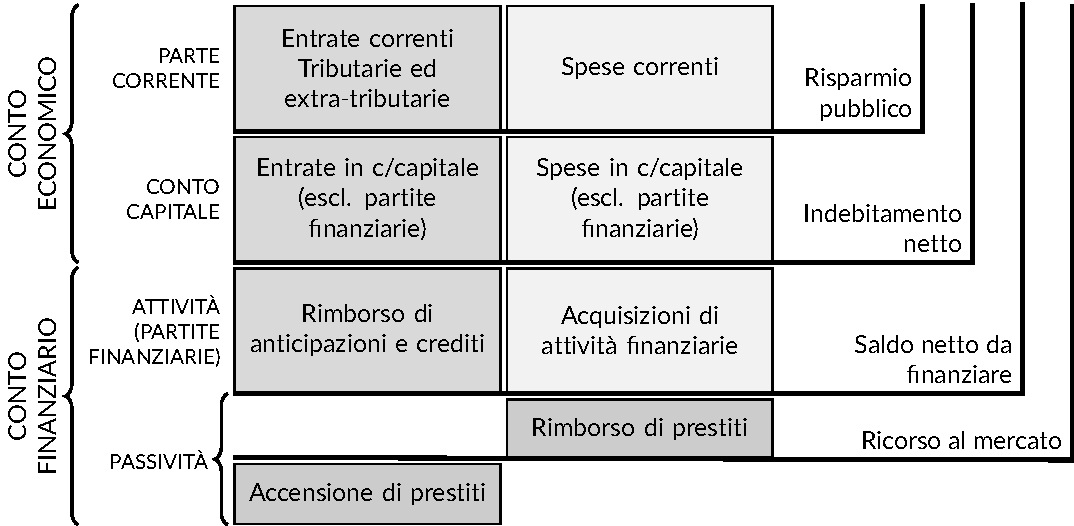
\includegraphics[width=12cm]{./figure/saldi-di-bilancio.pdf}
  \end{figure}
\end{frame}

%%%%%%%%%%%%%%%%%%%%%%%%%%%%%%%%%%%%%%%%%%%%
\begin{frame}{L'indebitamento netto nei principali paesi UE}
  \begin{figure}
    \centering
    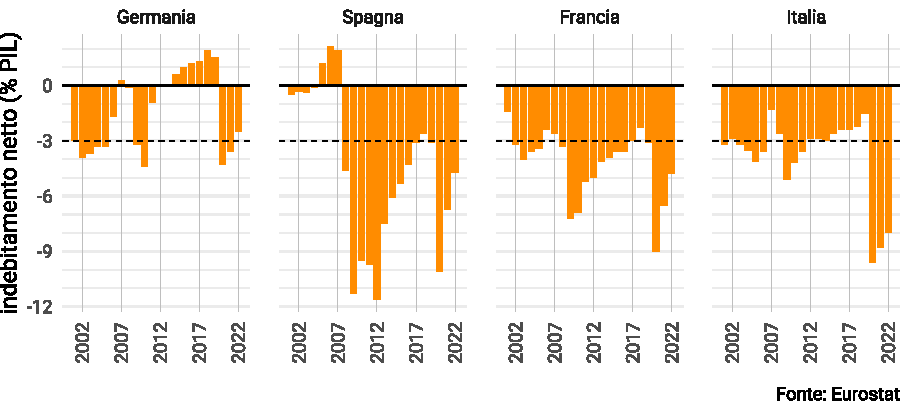
\includegraphics[width=\textwidth]{./figure/deficit-4countries-2000-2022-color.pdf}
  \end{figure}
\end{frame}


%%%%%%%%%%%%%%%%%%%%%%%%%%%%%%%%%%%%%%%%%%%%
\begin{frame}{È giustificabile la spesa in deficit?}

  \begin{itemize}
  \item Spese in eccesso sulle entrate correnti si possono giustificare:
    \begin{itemize}
    \item con la necessità di effettuare \alert{investimenti} finalizzati ad
      aumentare lo stock di capitale pubblico (es. infrastrutture);
    \item con l'esigenza di stabilizzare l'economia in presenza di
      fluttuazioni cicliche o eventi eccezionali (es. terremoti, alluvioni,
      guerre, pandemie), anche al fine di evitare che la capacità produttiva
      possa essere compromessa
    \end{itemize}
  \item In questi casi le imposte correnti potrebbero essere insufficienti a
    fronteggiare le necessità.
  \item Il deficit può essere un modo per rilanciare la domanda in un'ottica
    keynesiana.
  \item Può essere «giusto» sincronizzare il pagamento delle imposte e il
    godimento dei benefici di investimenti che hanno effetti di lungo periodo.
  \item In presenza di necessità di spesa concentrate nel tempo, ottimale
    distribuirne il peso in termini di riduzione dei consumi, in modo più
    uniforme nel tempo.
  \item \alert{Tuttavia}, la possibilità di rinviare nel tempo il pagamento
    delle imposte può avere effetti deresponsabilizzanti sui governi.
  \end{itemize}
\end{frame}

%%%%%%%%%%%%%%%%%%%%%%%%%%%%%%%%%%%%%%%%%%%%
\begin{frame}{Il dibattito sulla natura del debito pubblico}

  L'analogia con il debito di un privato può essere fuorviante per una
  pluralità di ragioni:
  \begin{enumerate}
  \item lo Stato, che ha vita virtualmente infinita, non ha necessità di
    restituire il debito, può continuare a rinnovarlo (\emph{rollover});
  \item lo Stato può, in caso di necessità, ripagare il debito creando moneta
    \begin{itemize}
    \item controindicazioni: inflazione, perdita di credibilità
    \end{itemize}
  \item spesso lo Stato si indebita con i propri cittadini, che sono ad un
    tempo creditori (in quanto possessori di titoli di Stato) e debitori (in
    quanto contribuenti);
  \item il debito non è «pagato» dalle generazioni future: le risorse per
    realizzare la spesa finanziata a debito sono distolte da quelle
    disponibili oggi
    \begin{itemize}
    \item «Non possiamo combattere le battaglie di oggi con i cavalli di
      domani»
    \item È un debito che «la mano destra deve alla mano sinistra»
    \end{itemize}
  \item C'è differenza tra debito interno e debito estero
  \end{enumerate}
\end{frame}

%%%%%%%%%%%%%%%%%%%%%%%%%%%%%%%%%%%%%%%%%%%%
\begin{frame}{Il dibattito sulla natura del debito pubblico /2}

  \begin{quoting}
    \small «Se si costruisce una ferrovia dal costo di 100 milioni,
    forsechè il terreno sarà stato spianato, i terrapieni innalzati, i ponti
    costruiti, le gallerie forate, le stazioni erette, i binari lanciati con
    lavoro e con materiale futuro?  Mai no. Che cosa è il costo della
    ferrovia, se non la fatica durata nello spianar terreni, innalzar
    terrapieni, forar gallerie, costruire ponti, fabbricare traversine rotaie
    locomotive carrozze e carri? Chi durò quella fatica?  I posteri od i
    viventi? […] Non esiste nessun mezzo per far sostenere ai posteri il
    costo, la fatica, il dolore di nessuna spesa presente. Se noi vivi
    vogliamo fare una spesa dobbiamo pagarcela noi con i mezzi presenti,
    dobbiamo volgere a quello scopo i mezzi che sarebbero disponibili per
    raggiungere altri fini presenti.»

    (L. Einaudi, 1940)
  \end{quoting}
\end{frame}

%%%%%%%%%%%%%%%%%%%%%%%%%%%%%%%%%%%%%%%%%%%%
\begin{frame}{Il dibattito sulla natura del debito pubblico /3}

  Tuttavia, la presenza di un debito rappresenta un costo:
  \begin{itemize}
  \item raccogliere le imposte per pagare gli interessi vincola la politica
    economica e impone un costo all'economia in futuro;
  \item il ricorso al debito potrebbe modificare le scelte di risparmio e
    accumulazione di capitale.
  \item Il debito pubblico rappresenta ricchezza per i privati?
    \begin{itemize}
    \item A un estremo potremmo rispondere di no, se i privati anticipano
      correttamente il fatto che dovranno finanziare il debito con le proprie
      imposte (equivalenza ricardiana).
    \item Se manca tale capacità di anticipazione, l'emissione di debito
      potrebbe ridurre il risparmio privato e determinare una riduzione della
      dotazione di capitale privato.
    \item In ottica keynesiana, al contrario, la spesa a debito potrebbe
      stimolare l'economia e indurre maggiori investimenti privati.
    \end{itemize}
  \end{itemize}
\end{frame}

%%%%%%%%%%%%%%%%%%%%%%%%%%%%%%%%%%%%%%%%%%%%
\begin{frame}{L'equivalenza ricardiana}

  \begin{itemize}
  \item Il debito pubblico rappresenta ricchezza per i privati? L'argomento
    tradizionale di Ricardo è che il finanziamento a debito equivale al
    finanziamento con un'imposta sul patrimonio corrente (vedi
    \emph{capitalizzazione} dell'imposta).
  \item Barro (1974) ha ripreso questo argomento: individui razionali, non
    soggetti a illusione finanziaria, anticipano il fatto che l'emissione del
    debito comporterà in futuro il pagamento di imposte.
  \item Il debito pubblico non è percepito come ricchezza in quanto
    interamente compensato dal valore attuale delle imposte future.
  \item Gli individui rispondono all'emissione di debito riducendo i propri
    consumi (aumentando il risparmio). Ciò vale anche quando le imposte
    saranno pagate dai discendenti, la cui utilità è «internalizzata» dalla
    generazione presente.
  \item L'argomento è stato utilizzato per contestare che la tesi keynesiana
    per cui spesa in deficit ha effetti espansivi sull'economia.
  \end{itemize}
\end{frame}

%%%%%%%%%%%%%%%%%%%%%%%%%%%%%%%%%%%%%%%%%%%%
\begin{frame}{Il debito pubblico nella contabilità nazionale}

  Ai fini della contabilità nazionale il debito pubblico rappresenta un
  sottoinsieme delle passività della Pubblica amministrazione. È rappresentato da:
  \begin{enumerate}
  \item biglietti monete e depositi (sono incluse le monete metalliche, non le
    banconote emesse dalla Banca centrale);
  \item titoli diversi da azioni e derivati;
  \item prestiti.
  \end{enumerate}
  Dal debito pubblico sono esclusi:
  \begin{itemize}
  \item debiti delle imprese pubbliche al di fuori del perimetro della
    P.A. (sono invece inclusi i titoli di Stato nel bilancio di tali imprese);
  \item i «crediti commerciali» della P.A. verso i fornitori;
  \item le garanzie esplicite o implicite fornite dallo Stato;
  \item il debito pensionistico.
\end{itemize}
Infine, il debito si considera comunemente al \emph{lordo} di eventuali
attività.
\end{frame}

%%%%%%%%%%%%%%%%%%%%%%%%%%%%%%%%%%%%%%%%%%%%
\begin{frame}{Il debito pubblico in alcuni paesi europei}
  
  \begin{figure}
    \centering
    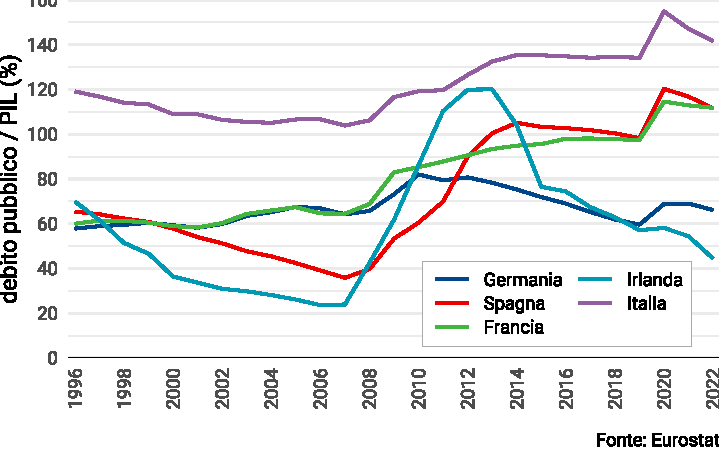
\includegraphics[width=.9\textwidth]{./figure/debito-eu-color.pdf}
  \end{figure}
\end{frame}

\section{L'aritmetica del debito pubblico}

%%%%%%%%%%%%%%%%%%%%%%%%%%%%%%%%%%%%%%%%%%%%
\begin{frame}{L'evoluzione del debito pubblico in funzione di deficit e crescita}

  \begin{itemize}
  \item Se trascuriamo la possibilità di finanziare il deficit aumentando il
    debito monetario (\emph{signoraggio}), vale la relazione:
    \begin{equation*}
      \Delta B_{t}=B_{t}-B_{t-1}= D_{t}
    \end{equation*}
    dove $B_{t}$ è lo stock di debito al termine del periodo $t$, $D_{t}$ è il
    deficit nel periodo $t$
  \item dividendo per $Y_{t}$ (tutte le variabili in \% del PIL) abbiamo
    \begin{equation*}
      \frac{B_{t}}{Y_{t}}=\frac{B_{t-1}}{Y_{t-1}(1+n)}+\frac{D_{t}}{Y_{t}}
      \quad\implies\quad
      b_{t}=\frac{b_{t-1}}{1+n}+d_{t}
    \end{equation*}
    dove $b_t=B_{t}/Y_{t}$ e $d_{t}=D_{t}/Y_{t}$. Ricordiamo che
    $Y_{t}=Y_{t-1}(1+n)$.
  \item Fissando $n$ e $d$, la dinamica di $Y_{t}/B_{t}$ può essere illustrata
    con l'aiuto di un
    \href{https://docs.google.com/spreadsheets/d/1taAlA7ksKNweRqOguMfEDdVAYOXU3TlYrjClW6MumaE/edit?usp=sharing}%
    {→foglio elettronico}: osserviamo che al crescere di $t$ il rapporto
    converge ad un valore che dipende da $d$ e da $n$
  \end{itemize}
\end{frame}

%%%%%%%%%%%%%%%%%%%%%%%%%%%%%%%%%%%%%%%%%%%%
\begin{frame}{L'aritmetica del debito: il rapporto debito/PIL in funzione di
    $d$ e $n$}

  \begin{columns}
    \begin{column}{.5\columnwidth}
      \begin{itemize}
      \item Fissando un livello di deficit e mantenendolo costante
        ($d_{t}=d$), abbiamo la dinamica descritta in figura
      \item il valore di equilibrio si ottiene ponendo $b_{t}=b_{t-1}=b^*$
        nella
        \begin{equation*}
          b_{t}=\frac{b_{t-1}}{1+n}+d_{t}
        \end{equation*}
        ovvero:
        \begin{equation*}
          b^*=\frac{1+n}{n}\cdot d \approx \frac{d}{n}
        \end{equation*}
      \item l'equilibrio è stabile se $n>0$
      \end{itemize}
    \end{column}

    \begin{column}{.5\columnwidth}
      \begin{figure}
        \centering
        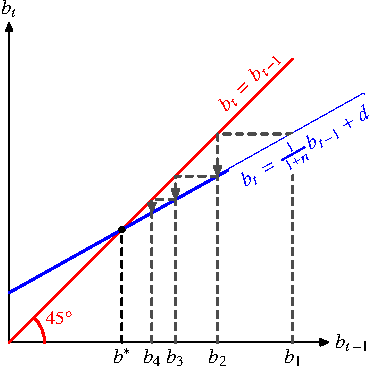
\includegraphics[width=\textwidth]{./figure/debito-pubblico-sost-1.pdf}
      \end{figure}
    \end{column}
  \end{columns}
  
\begin{block}{}
  I parametri di Maastricht ($b=60\%$ e $d=3\%$) sono coerenti se $n=5\%$,
  ovvero, visto che $n\approx g + \pi$, con crescita reale $g=3\%$ e
  inflazione $\pi=2\%$
\end{block}

\end{frame}

%%%%%%%%%%%%%%%%%%%%%%%%%%%%%%%%%%%%%%%%%%%%
\begin{frame}{L'aritmetica del debito: l'avanzo primario che stabilizza il debito}
  
  \begin{itemize}
  \item Scomponiamo il deficit in spesa per interessi e \alert{avanzo primario}:
    \begin{equation*}
      D_{t}=iB_{t-1}-(T_{t}-G_{t}) 
      \quad\implies\quad 
      d_{t}=\frac{ib_{t-1}}{1+n}-a_{t}
    \end{equation*}
    dove $a_{t}=(T_{t}-G_{t})/Y_{t}$ è l'avanzo primario in percentuale del PIL.
  \item Abbiamo dunque
    \begin{equation*}
      b_{t} = \frac{b_{t-1}}{1+n} + \frac{ib_{t-1}}{1+n} - a_{t}.
    \end{equation*}
  \item Fissando $b_{t}=b_{t-1}$, possiamo calcolare \alert{il livello di
      $a_{t}$ necessario a stabilizzare il debito}. Abbiamo:
    \begin{equation*}
      a_{t} = \left(\frac{i-n}{1+n}\right)b_{t-1} \; \approx (i-n)b_{t-1}.
    \end{equation*}
    \begin{itemize}
    \item Se $n=0$ (crescita zero), deve essere $a_{t}=ib_{t-1}$;
    \item $\frac{i-n}{1+n}$ è spesso indicato come \emph{tasso di interesse
        aggiustato per la crescita};
    \item se $a_t$ è maggiore (minore) di $\frac{i-n}{1+n}b_{t-1}$ il livello
      di $b$ decresce (cresce);
    \item l'avanzo primario necessario per stabilizzare il debito è tanto
      maggiore quanto più alto è $b_{t-1}$, quanto più alto è $i$ e quanto più
      bassa è la crescita $n$.
    \end{itemize}
  \end{itemize}
\end{frame}

%%%%%%%%%%%%%%%%%%%%%%%%%%%%%%%%%%%%%%%%%%%%
\begin{frame}{Le determinanti della crescita del debito}

  \begin{itemize}
  \item Possiamo identificare le determinanti della crescita di $b$ scrivendo
    \begin{equation*}
      b_{t}-b_{t-1}=\frac{i}{1+n}b_{t-1}-\frac{n}{1+n}b_{t-1}+a_{t}
      \;\;\approx (i-n)b_{t-1}-a_{t}
    \end{equation*}
    per cui la variazione di $b$ dipende positivamente dal tasso di interesse
    $i$ e negativamente dal tasso di crescita $n$ e dall'avanzo primario $a$
  \item In sintesi, la dinamica del debito dipende da tre variabili: l'avanzo
    primario $a_t$, il tasso di interesse $i$ e il tasso di crescita $n$.
  \item Notiamo che:
    \begin{itemize}
    \item quando $i>n$ è necessario un saldo primario $a_t$ positivo per
      stabilizzare il debito
    \item quando $n>i$ la dinamica del debito è stabile, è sufficiente fissare
      $a_t$ per avere convergenza.
    \end{itemize}
  \item Un problema è dato dal fatto che $a$ può influenzare sia $n$ che $i$.
  \end{itemize}
\end{frame}

%%%%%%%%%%%%%%%%%%%%%%%%%%%%%%%%%%%%%%%%%%%%
\begin{frame}{L'evoluzione del debito italiano e le sue determinanti}

  \begin{figure}
    \centering
    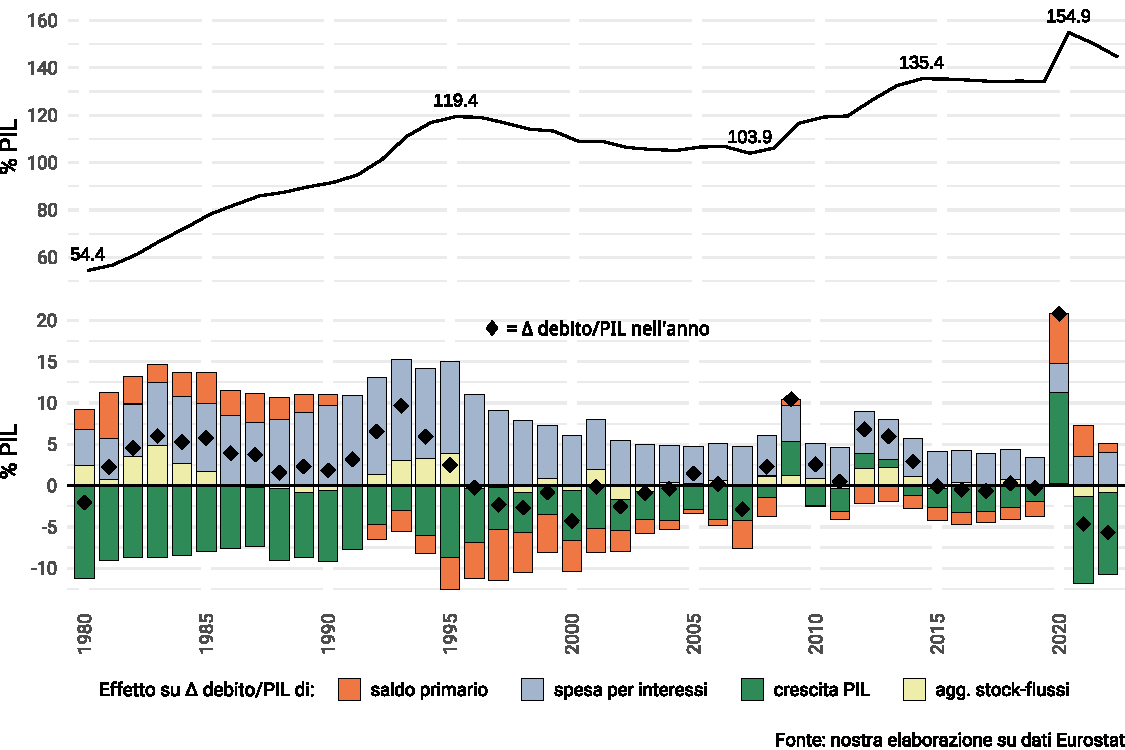
\includegraphics[width=.9\textwidth]{./figure/crescita-debito-1980-2024-scomposizione-nominale-color.pdf}
  \end{figure}
\end{frame}

%%%%%%%%%%%%%%%%%%%%%%%%%%%%%%%%%%%%%%%%%%%%
\begin{frame}{L'evoluzione del debito italiano e le sue determinanti /2}

  Alcune osservazioni:
  \begin{itemize}
  \item L'attuale situazione di debito elevato si è creata principalmente nel
    corso degli anni '80. Il rapporto debito/PIL si è ridotto a partire da
    metà anni '90 ed è tornato a crescere con la crisi
  \item Le fasi di crescita rapida del debito sembrano dipendere più
    dall'andamento della componente $(i-n)b_{t-1}$ che dall'avanzo primario,
    che è rimasto positivo dopo il 1992
    \begin{itemize}
    \item Negli anni '70 deficit primari anche elevati, ma l'elevata crescita
      nominale (superiore al tasso di interesse) evitava un aumento rapido del
      debito
    \item Negli anni '80 rallentamento della crescita nominale, elevati tassi
      di interesse (liberalizzazione dei mercati dei capitali e politica
      monetaria USA) e deficit in calo solo alla fine del periodo
    \item Nei primi anni '90 consistente consolidamento fiscale
    \item A fine anni '90 riduzione dei tassi di interesse per effetto della
      stabilizzazione del cambio e dell'ingresso nell'euro
    \item Con la crisi l'effetto è principalmente quello della crescita bassa
      o negativa, nonostante lo sforzo di consolidamento
    \end{itemize}
  \end{itemize}
\end{frame}

%%%%%%%%%%%%%%%%%%%%%%%%%%%%%%%%%%%%%%%%%%%%
\begin{frame}{L'evoluzione del debito italiano e le sue determinanti /3}

  \begin{itemize}
  \item Il grafico illustra l'andamento di $n$ (crescita del PIL nominale) e
    $i$ (tasso di interesse medio sulle emissioni di titoli di Stato)
  \end{itemize}

  \begin{figure}
    \centering
    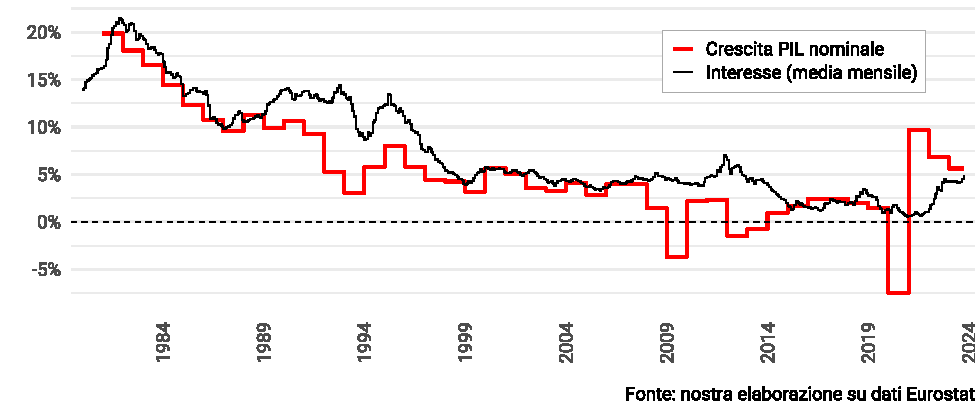
\includegraphics[width=\textwidth]{./figure/interesse-crescita-Italy-color.pdf}
  \end{figure}
\end{frame}

%%%%%%%%%%%%%%%%%%%%%%%%%%%%%%%%%%%%%%%%%%%%
\begin{frame}{Insolvenza e sostenibilità del debito}

  \begin{itemize}
  \item Si parla di \alert{insolvenza} se lo Stato non è in condizioni di
    onorare i propri impegni (pagare gli interessi, rimborsare i titoli a
    scadenza\ldots{})
  \item Si parla di \alert{default} se lo Stato non paga interessi e titoli a
    scadenza: il default può essere volontario, a prescindere dalla capacità
    di pagare.
  \item Una \alert{ristrutturazione} del debito è una modifica, solitamente
    negoziata coi creditori, delle scadenze e dei pagamenti.
  \item La \alert{solvibilità} non è facile da determinare in concreto. Si
    preferisce parlare di \alert{sostenibilità} del debito. La sostenibilità
    corrisponde a un'elevata probabilità che uno Stato risulti solvibile.
  \item La solvibilità è influenzata da:
    \begin{itemize}
    \item struttura per scadenze dei titoli di Stato;
    \item identità dei creditori: se sono risparmiatori, investitori
      istituzionali, organizzazioni internazionali, altri Stati\ldots{}
    \item valuta di denominazione del debito (es. molti paesi economicamente
      meno avanzati si indebitano in dollari o altra valuta): ciò espone il
      paese al rischio di una crisi della bilancia dei pagamenti e alle
      fluttuazioni del tasso di cambio.
    \end{itemize}
  \end{itemize}
\end{frame}

%%%%%%%%%%%%%%%%%%%%%%%%%%%%%%%%%%%%%%%%%%%%
\begin{frame}{Fattori che incidono sulla sostenibilità del debito}

  \begin{itemize}
  \item Se fossimo in grado di identificare il livello massimo di avanzo
    primario \(\hat a\), il limite sarebbe
    \begin{equation*}
      \hat{b}=\frac{1+n}{i-n}\hat{a}
    \end{equation*}
    visto che un livello di \(b\) superiore non potrebbe essere «stabilizzato»
    e quindi si determinerebbe una dinamica divergente del rapporto
    debito/PIL.
  \item Tuttavia, non è ovvio cosa possa limitare la capacità di fissare \(a\)
    al livello necessario. Non è solo questione di capacità, anche di volontà
    politica.
  \item L'analisi della sostenibilità deve tenere conto dei possibili
    shock. Tra essi:
    \begin{itemize}
    \item shock macroeconomici
    \item cambiamenti delle aspettative degli investitori.
    \end{itemize}
  \end{itemize}
\end{frame}

%%%%%%%%%%%%%%%%%%%%%%%%%%%%%%%%%%%%%%%%%%%%
\begin{frame}{Quali politiche per la riduzione del debito?}

  \begin{itemize}
  \item Crescita economica (aumentare $g$)
  \item Realizzazione di avanzi primari (aumentare $a$) riducendo le spese o
    aumentando le imposte
  \item Inflazione non anticipata (aumentare $\pi$, e quindi $n$, senza
    aumentare $i$)
  \item "Repressione finanziaria" (ridurre $i$) incoraggiando o forzando
    l'acquisto di titoli di stato da parte di intermediari finanziari o
    famiglie
  \item Default del debito
  \end{itemize}

  Ovviamente, non tutte queste strade sono equivalenti. Alcune di esse possono
  non essere attuabili o possono comportare costi elevati per il Paese.
\end{frame}

%%%%%%%%%%%%%%%%%%%%%%%%%%%%%%%%%%%%%%%%%%%%
\begin{frame}{Il debito italiano dall'Unità d'Italia al 2017}

  \begin{figure}
    \centering
    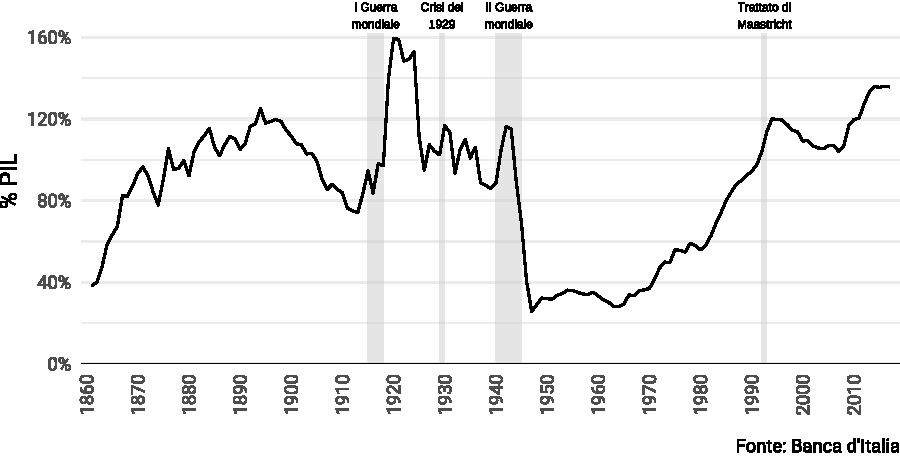
\includegraphics[width=\textwidth]{./figure/debito-PIL-1861-2017.pdf}
  \end{figure}
\end{frame}


%%%%%%%%%%%%%%%%%%%%%%%%%%%%%%%%%%%%%%%%%%%%
\begin{frame}{L'inflazione e il debito}
  
  \begin{itemize}
  \item Consideriamo l'effetto di un aumento dell'inflazione $\pi$:
    \begin{itemize}
    \item l'aumento dei prezzi si riflette direttamente sulla
      crescita nominale:  $1+n^*=(1+n)(1+\pi)$
    \item nella misura in cui è anticipata ($\pi^e$), la maggiore inflazione si riflette sui
      tassi di interesse $1+i\,^*=(1+i)(1+\pi^e)$
    \end{itemize}
  \item Calcoliamo dunque i nuovi valori dei tassi di interesse e di crescita:
    \begin{equation*}
      \frac{i\,^*-n^*}{1+n^*} = \frac{1+i\,^*}{1+n^*}-1 = \frac{(1+i)(1+\pi^e)}{(1+n)(1+\pi)}-1
    \end{equation*}
  \item Quando $\pi^e<\pi$ (l'inflazione non è interamente anticipata):
    \begin{equation*}
      \frac{i\,^*-n^*}{1+n^*} < \frac{i-n}{1+n}.
    \end{equation*}
  \end{itemize}
\end{frame}


\section{I vincoli alla politica di bilancio}

%%%%%%%%%%%%%%%%%%%%%%%%%%%%%%%%%%%%%%%%%%%%
\begin{frame}{Le ragioni dei limiti di bilancio}

  \begin{itemize}
  \item I politici tendono a operare in un orizzonte di breve periodo e
    l'elettorato è poco informato o è, a sua volta, «miope» rispetto agli
    effetti di lungo periodo delle scelte politiche.
  \item I beneficiari delle spese sono spesso gruppi limitati di individui,
    mentre il debito si ripartisce sulla collettività e sulle generazioni
    future.
  \item In un'unione monetaria i singoli paesi possono essere
    deresponsabilizzati dalla prospettiva di un intervento della Banca
    centrale a sostegno del debito. A questo riguardo, le clausole che vietano
    il finanziamento diretto dei debiti e la proibizione di «accesso
    privilegiato» alle isstituzioni finanziarie non sembrano deterrenti
    sufficienti.
  \end{itemize}
  
\begin{block}{}
  La crisi del 2008 ha tuttavia mostrato come troppa poca attenzione fosse
  stata posta ai \alert{debiti privati}, per salvare i quali molti paesi hanno
  compromesso le rispettive posizioni debitorie «sane» (es. Irlanda e Spagna),
  e agli \alert{squilibri della bilancia dei pagamenti}
\end{block}
\end{frame}

%%%%%%%%%%%%%%%%%%%%%%%%%%%%%%%%%%%%%%%%%%%%
\begin{frame}{L'equilibrio di bilancio: la Costituzione}
  
  Nel 2012, a seguito degli impegni internazionali presi con il \alert{fiscal
    compact}, il Parlamento ha modificato l'art. 81 della Costituzione,
  introducendo il principio dell'\alert{equilibrio di bilancio}. Al Comma 1:

  \begin{quoting}
    \footnotesize Lo Stato assicura l’equilibrio tra le entrate e le spese del
    proprio bilancio, tenendo conto delle fasi avverse e delle fasi favorevoli
    del ciclo economico.

    Il ricorso all’indebitamento è consentito solo al fine di considerare gli
    effetti del ciclo economico e, previa autorizzazione delle Camere adottata
    a maggioranza assoluta dei rispettivi componenti, al verificarsi di eventi
    eccezionali.
  \end{quoting}

  Il Comma 6 dell'Art. 81 rinvia, per i criteri, a una legge approvata con
  maggioranza qualificata. La L. 243/2012 per l'attuazione del «pareggio di
  bilancio» identifica l'equilibrio con il conseguimento dell'\alert{obiettivo
    di medio termine}, ovvero:

  \begin{quoting}
    \small «il valore del \alert{saldo strutturale} individuato sulla base dei
    criteri stabiliti dall'ordinamento dell'Unione europea».
  \end{quoting}

  La legge rinvia in modo esplicito al \alert{Patto di stabilità e crescita}
  della UE.
\end{frame}


%%%%%%%%%%%%%%%%%%%%%%%%%%%%%%%%%%%%%%%%%%%%
\begin{frame}{Il Patto di Stabilità e Crescita}
  
  \begin{itemize}
  \item Il quadro di riferimento europeo per le politiche di bilancio è dato
    dal \alert{Patto di Stabilità e Crescita} (\emph{Stability and Growth Pact
      -- SGP}), sottoscritto nel 1997 e successivamente rafforzato. Esso
    prevede
    \begin{itemize}
    \item un \alert{braccio preventivo}, alla base del quale c'è la
      definizione per ciascun paese di uno specifico \alert{obiettivo di medio
        termine} (\emph{medium term objective - MTO})
    \item un \alert{braccio correttivo} reso operativo dalla \alert{Procedura
        per deficit eccessivo} (\emph{Excessive Deficit Procedure – EDP}) che
      si applica in caso di violazione della regola del deficit o di quella
      del debito
    \end{itemize}
  \end{itemize}
  \begin{block}{Le basi normative}
    \scriptsize\addtolength{\itemsep}{-10pt}
    \begin{itemize}
    \item gli articoli
      →\href{http://eur-lex.europa.eu/LexUriServ/LexUriServ.do?uri=CELEX:12008E121:EN:NOT}{121}
      e
      →\href{http://eur-lex.europa.eu/LexUriServ/LexUriServ.do?uri=CELEX:12008E126:EN:NOT}{126}
      del Trattato (TFEU)
    \item il
      →\href{http://europa.eu/legislation\_summaries/economic\_and\_monetary\_affairs/stability\_and\_growth\_pact/l25019\_en.htm}{Regolamento
        1466/97} e relative modifiche
    \item il \alert{Six Pack}, in vigore dal 13/12/2011, che riforma e
      rafforza la legislazione secondaria, introducendo il \alert{semestre
        europeo}
    \item il \alert{Fiscal compact}, contenuto nel trattato intergovernativo
      (vincolante per chi lo ha sottoscritto e per chi adotterà l'euro) su
      stabilità, coordinamento e governance (TSCG) in vigore dal 1/1/2013
    \item il \alert{Two Pack}, in vigore dal 30/5/2013, che introduce
      ulteriori strumenti di sorveglianza e monitoraggio
\end{itemize}
→\href{http://ec.europa.eu/economy\_finance/economic\_governance/sgp/legal\_texts/index\_en.htm}{Stability
  and Growth Pact sul sito della Commissione}
\end{block}
\end{frame}

%%%%%%%%%%%%%%%%%%%%%%%%%%%%%%%%%%%%%%%%%%%%
\begin{frame}{Gli effetti del ciclo sul saldo di bilancio}

  \begin{itemize}
  \item Il ciclo economico influenza i saldi di finanza pubblica. Infatti:
    \begin{itemize}
    \item il livello di attività economica influenza le entrate fiscali e, in
      certa misura, la spesa pubblica (vedi sussidi di disoccupazione): in
      situazioni di crisi l'operare di \alert{stabilizzatori automatici} crea
      un deficit anche a legislazione invariata
    \item i saldi sono definiti in \% del PIL, a parità di entrate/uscita il
      rapporto risente di variazioni del PIL
    \end{itemize}
  \item Il saldo di bilancio (lo indichiamo come «saldo effettivo» per
    distinguerlo dal «saldo strutturale») è:
    \begin{equation*}
      \text{saldo effettivo}\quad s(Y)=\frac{T(Y)-G(Y)}{Y}
    \end{equation*}
    con $T(Y)$ decrescente e $G(Y)$ crescente rispetto al reddito, $s(Y)$ è
    funzione crescente di $Y$.
  \item Perseguire il pareggio di bilancio in una recessione rappresenta una manovra
    \alert{prociclica}, che può accentuare la riduzione del PIL.
  \end{itemize}
\end{frame}

%%%%%%%%%%%%%%%%%%%%%%%%%%%%%%%%%%%%%%%%%%%%
\begin{frame}{Saldo effettivo e saldo strutturale}

  \begin{itemize}
  \item Indichiamo con $s(Y^*)$ il \alert{saldo strutturale}, che si otterrebbe in
    corrispondenza del livello del PIL in piena occupazione (o PIL potenziale)
    $Y^*$. Chiaramente: $s(Y)>s(Y^*)$ se e solo se $Y>Y^*$.
  \item Ipotizzando che $T(Y)=tY$ e $G(Y)=G^*$, abbiamo:
    \begin{equation*}
      s(Y)=\frac{tY - G^*}{Y} \quad\implies\quad s'(Y)=\frac{G^*}{Y^2}
    \end{equation*}
  \item Dunque:
    \begin{equation*}
      s(Y)\approx s(Y^*)+(Y-Y^*)s'(Y^*)=s(Y^*)+\frac{Y-Y^*}{Y^*}\frac{G^*}{Y^*}
    \end{equation*}
    dove $\frac{Y-Y^*}{Y^*}$ è detto \emph{output gap} e $G^*/Y^*$ varia da paese a
    paese in base alla dimensione della spesa pubblica. In Italia è 0,55.
    \begin{equation*}
      \text{[saldo strutturale]} =
         \text{[saldo corrente]} -  0,\!55 \times\text{[output gap]}
    \end{equation*}
  \item Quando l'economia è sotto il suo potenziale (\emph{output gap}
    negativo) il saldo strutturale risulta dunque migliore del saldo
    effettivo. Il perseguimento del pareggio strutturale riduce la necessità
    di manovre procicliche.
  \end{itemize}
\end{frame}


%%%%%%%%%%%%%%%%%%%%%%%%%%%%%%%%%%%%%%%%%%%%
\begin{frame}{Il «braccio preventivo» del Patto di stabilità e crescita}

  \begin{itemize}
  \item \alert{Obiettivo di medio termine}: prevede che il paese sia in
    pareggio strutturale o \emph{prossimo al} pareggio strutturale, o sia su
    un sentiero di convergenza verso tale obiettivo.
  \item Il raggiungimento dell'obiettivo è rafforzato dalla \alert{regola
      della spesa}, che prevede un limite alla crescita annua della spesa
    pubblica \alert{primaria}, calcolata al netto di alcune spese legate al
    ciclo (es. sussidi di disoccupazione) e della spesa per i programmi
    europei.
    \begin{itemize}
    \item La spesa può essere aumentata oltre tale limite solo in presenza di
      un aumento corrispondente delle entrate (un aumento «discrezionale»,
      cioè dovuto a un esplicito cambiamento legislativo, non automatico).
    \item Il limite di crescita della spesa è pari alla crescita media del PIL
      potenziale, corretta da un fattore che dipende dalla distanza
      dall'obiettivo di medio termine.
    \end{itemize}
  \item Il mancato rispetto di tali obiettivi comporta l'avvio di una
    \alert{procedura per deviazione significativa} (\emph{Significant
      Deviation Procedure}), con l'obbligo per il Paese di attuare azioni
    correttive, pena l'applicazione di sanzioni.
  \end{itemize}
\end{frame}

%%%%%%%%%%%%%%%%%%%%%%%%%%%%%%%%%%%%%%%%%%%%
\begin{frame}{Il «braccio correttivo» del Patto di stabilità e crescita}

  Ciascun paese è tenuto inoltre a rispettare i vincoli su deficit corrente e
  debito fissati nel Trattato di Maastricht (Art. 126 TFUE):
  \begin{itemize}
  \item \alert{Limite al deficit corrente} (indebitamento netto): non può
    eccedere il 3\% del PIL, a meno che il superamento non sia eccezionale e
    temporaneo o non sia diminuito e in avvicinamento a tale valore.
  \item \alert{Limite al rapporto debito/PIL} che non deve superare il
    60\%. Si intende rispettato se tale rapporto si sta «riducendo in misura
    sufficiente» e si sta avvicinando al valore di riferimento «con ritmo
    adeguato»:
    \begin{itemize}
    \item \alert{Regola del debito}: la riduzione annua del rapporto
      debito/PIL deve essere almeno pari a 1/20 della differenza tra debito
      corrente e limite del 60\%.
    \end{itemize}
  \item Il mancato rispetto di tali limiti comporta l'apertura di una
    \alert{procedura per disavanzo eccessivo} (\emph{Excessive Deficit
      Procedure}, EDP). Anche in questo caso dovranno essere attuate azioni
    correttive, pena l'applicazione di sanzioni.
  \end{itemize}
  \begin{block}{}
    \small La decisione sull'apertura delle procedure di violazione non è
    automatica, spetta al Consiglio dei ministri dell'economia e finanze dei
    paesi UE (ECOFIN), su proposta della Commissione.
  \end{block}
\end{frame}

%%%%%%%%%%%%%%%%%%%%%%%%%%%%%%%%%%%%%%%%%%%%
\begin{frame}{La flessibilità dei vincoli europei}

  \begin{itemize}
  \item Le regole descritte non sono applicate in modo meccanico è rigido. È
    prevista una certa flessibilità per tenere conto di circostanze specifiche
    e consentire spazi fiscali per realizzare riforme:
    \begin{itemize}
    \item in presenza di recessione, a seconda della gravità della stessa, gli
      aggiustamenti di bilancio richiesti sono di entità inferiore;
    \item in presenza di «riforme strutturali» e programmi di investimenti
      approvati dalla UE è concesso un maggiore spazio di bilancio.
    \end{itemize}
  \item In presenza di situazioni eccezionali si possono sospendere
    temporaneamente le regole europee (\alert{clausola di salvaguardia
      generale})
    \begin{itemize}
    \item Tale clausola è stata applicata nella primavera del 2020. Per
      consentire di intraprendere le azioni energiche richieste dalla crisi
      pandemica, le regole del braccio correttivo e del braccio preventivo
      sono rimaste sospese fino a tutto il 2023.
    \end{itemize}
  \end{itemize}
\end{frame}

%%%%%%%%%%%%%%%%%%%%%%%%%%%%%%%%%%%%%%%%%%%%
\begin{frame}{La riforma del Patto di stabilità}

  \begin{itemize}
  \item Insoddisfazione per l'attuale sistema di regole:
    \begin{itemize}
    \item regole troppo complesse;
    \item troppa discrezionalità della Commissione e del Consiglio che conduce
      a una «politicizzazione» delle decisioni;
    \item regole uniformi per paesi con situazioni diverse.
    \end{itemize}
  \item Nello specifico:
    \begin{itemize}
    \item la stima dell'\emph{output gap} è soggetta ad ampi margini di errore
      e la stessa nozione di \emph{output gap} viene contestata dal punto di
      vista teorico. Al di là delle intenzioni, non si elimina l'effetto
      prociclico delle politiche di bilancio.
    \item le regole correnti, non distinguendo tra spese correnti e
      investimenti, finoscono per scoraggiare questi ultimi, più facilmente
      rinviabili. Sarebbe desiderabile una \alert{golden rule}, ovvero una
      regola che limitasse le sole spese correnti, escludendo dal vincolo le
      spese in conto capitale.
    \end{itemize}
  \end{itemize}
\end{frame}


%%%%%%%%%%%%%%%%%%%%%%%%%%%%%%%%%%%%%%%%%%%%
\begin{frame}{La riforma del Patto di stabilità /2}

  \begin{itemize}
  \item Il progetto di riforma attualmente in discussione:
    \begin{itemize}
    \item semplificazione, con adozione di un'unica regola, che ricalca la
      \alert{regola della spesa} ed è fissata in funzione dell'obiettivo di
      riduzione del debito pubblico.
    \item traiettorie di riduzione del debito definite Paese per Paese in base
      alla specifica situazione economica e fiscale;
    \item più spazio agli investimenti;
    \item più automatismo nel definire una violazione delle regole;
    \end{itemize}
  \end{itemize}

  \begin{figure}
    \centering
    \includegraphics[width=10cm]{./figure/titolo-Sole-su-patto-stabilità.png}
  \end{figure}
  \scriptsize \emph{Il Sole 24 Ore} del 9/12/23
\end{frame}

%%%%%%%%%%%%%%%%%%%%%%%%%%%%%%%%%%%%%%%%%%%%
\begin{frame}{Il «semestre europeo»}

  \begin{itemize}
  \item Introdotto nel 2010 per favorire il coordinamento a livello europeo
    preliminarmente alla programmazione di bilancio a livello nazionale:
    \begin{itemize}
    \item il quadro previsionale macroeconomico adottato dai diversi paesei è
      definito in modo omogeneo a livello europeo;
    \item si ha una valutazione preventiva degli obiettivi definiti dai paesi.
    \end{itemize}
  \end{itemize}

  \begin{figure}[htbp]
    \centering
    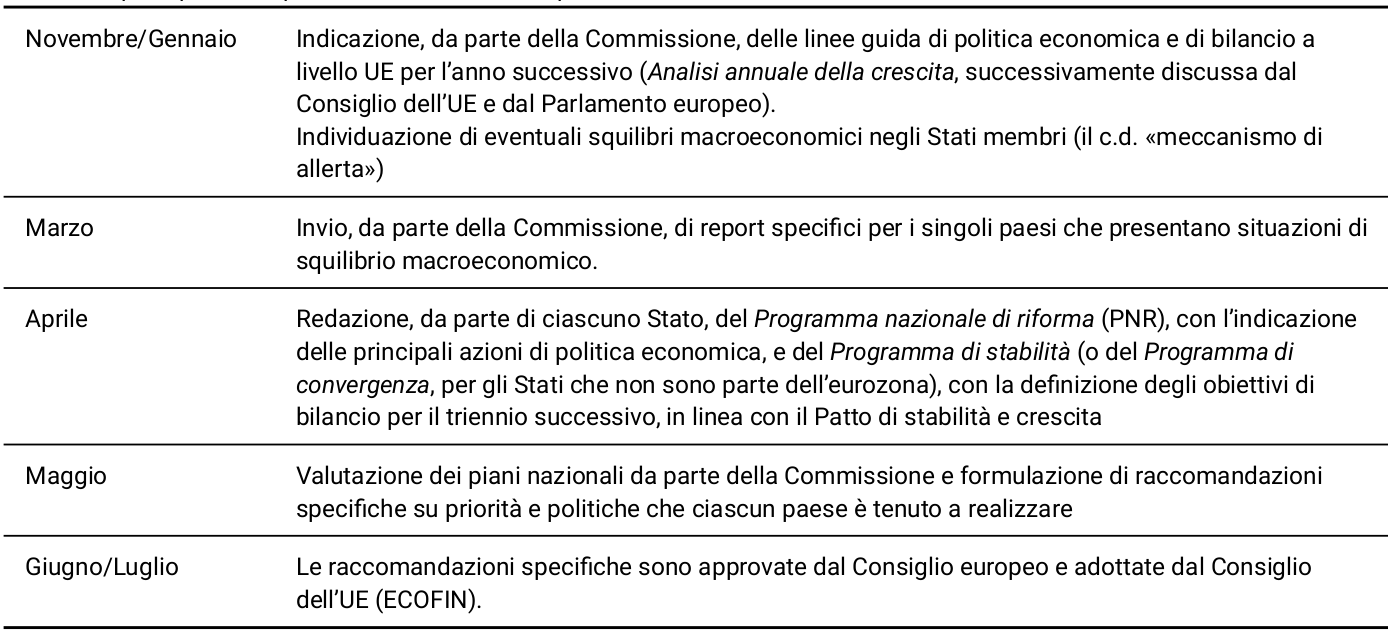
\includegraphics[height=5cm]{./figure/semestre-europeo.png}
  \end{figure}
\end{frame}


\section{Il ciclo di bilancio e la manovra di finanza pubblica}

%%%%%%%%%%%%%%%%%%%%%%%%%%%%%%%%%%%%%%%%%%%%
\begin{frame}{Il ciclo dei documenti di finanza pubblica (ex L. 196/2009, art. 7)}

  \begin{itemize}
  \item Il \alert{Documento di Economia e Finanza (DEF)}
    (→\href{http://www.mef.gov.it/documenti-pubblicazioni/doc-finanza-pubblica/index.html}{vedi sul sito del MEF})
    illustra la situazione economico-finanziaria del Paese e gli obiettivi che
    il Governo intende raggiungere. Comprende:
    \begin{itemize}
    \item \alert{Sez.I - Programma di Stabilità}. Indica il quadro delle
      previsioni economico-finanziarie e gli obiettivi relativi ai principali
      saldi di finanza pubblica per il triennio successivo
    \item \alert{Sez.II - Analisi e tendenze della finanza pubblica.} I conti
      pubblici dell'anno precedente e le previsioni, dettagliati per
      sottosettori di spesa
    \item \alert{Sez.III - Programma nazionale di riforma.} Indica lo stato di
      avanzamento delle riforme avviate, gli squilibri macroeconomici e i
      fattori che incidono sulla competitività, le riforme da attuare e il
      loro prevedibile impatto
    \end{itemize}
    È presentato alle Camere entro il 10 aprile, così da consentire l’approvazione
    e l’invio, entro il 30 aprile, delle sezioni relative al Programma di
    Stabilità (PS) e al Piano Nazionale di Riforma (PNR) al Consiglio dell’Ue.
  \end{itemize}
\end{frame}

%%%%%%%%%%%%%%%%%%%%%%%%%%%%%%%%%%%%%%%%%%%%
\begin{frame}{Il ciclo dei documenti di finanza pubblica (continua)}

  \begin{itemize}
  \item La \alert{Nota di aggiornamento al DEF} contiene gli eventuali
    aggiornamenti degli obiettivi programmatici fissati nel DEF anche al fine
    di recepire le raccomandazioni formulate dal Consiglio dell’Unione
    Europea. È presentata dal Governo al Parlamento entro il 20 settembre.
  \item Il \alert{Documento Programmatico di Bilancio (DPB)} riprende gli
    obiettivi programmatici contenuti nella Nota di aggiornamento al DEF ed
    illustra le misure inserite nella manovra di bilancio. È trasmesso entro
    il 15 ottobre
    alla Commissione Europea e all'Eurogruppo \\[0pt]
    \emph{In attuazione del Regolamento UE n.473/2013 (Two Pack)}
  \item Il \alert{DDL di Bilancio}. La sua presentazione entro il 15 ottobre
    dà inizio alla sessione parlamentare di bilancio. Deve essere approvato
    dal Parlamento entro il 31 dicembre.
  \item Il \alert{Rendiconto generale} rileva e riassume i risultati ottenuti
    nel corso dell’anno precedente. È presentato dal Governo al Parlamento per
    approvazione, previa verifica della Corte dei conti, entro il 30 giugno.
  \end{itemize}
\end{frame}

%%%%%%%%%%%%%%%%%%%%%%%%%%%%%%%%%%%%%%%%%%%%
\begin{frame}{I saldi di bilancio corretti per il ciclo}

  \vspace{-5mm}
  \begin{figure}
    \centering
    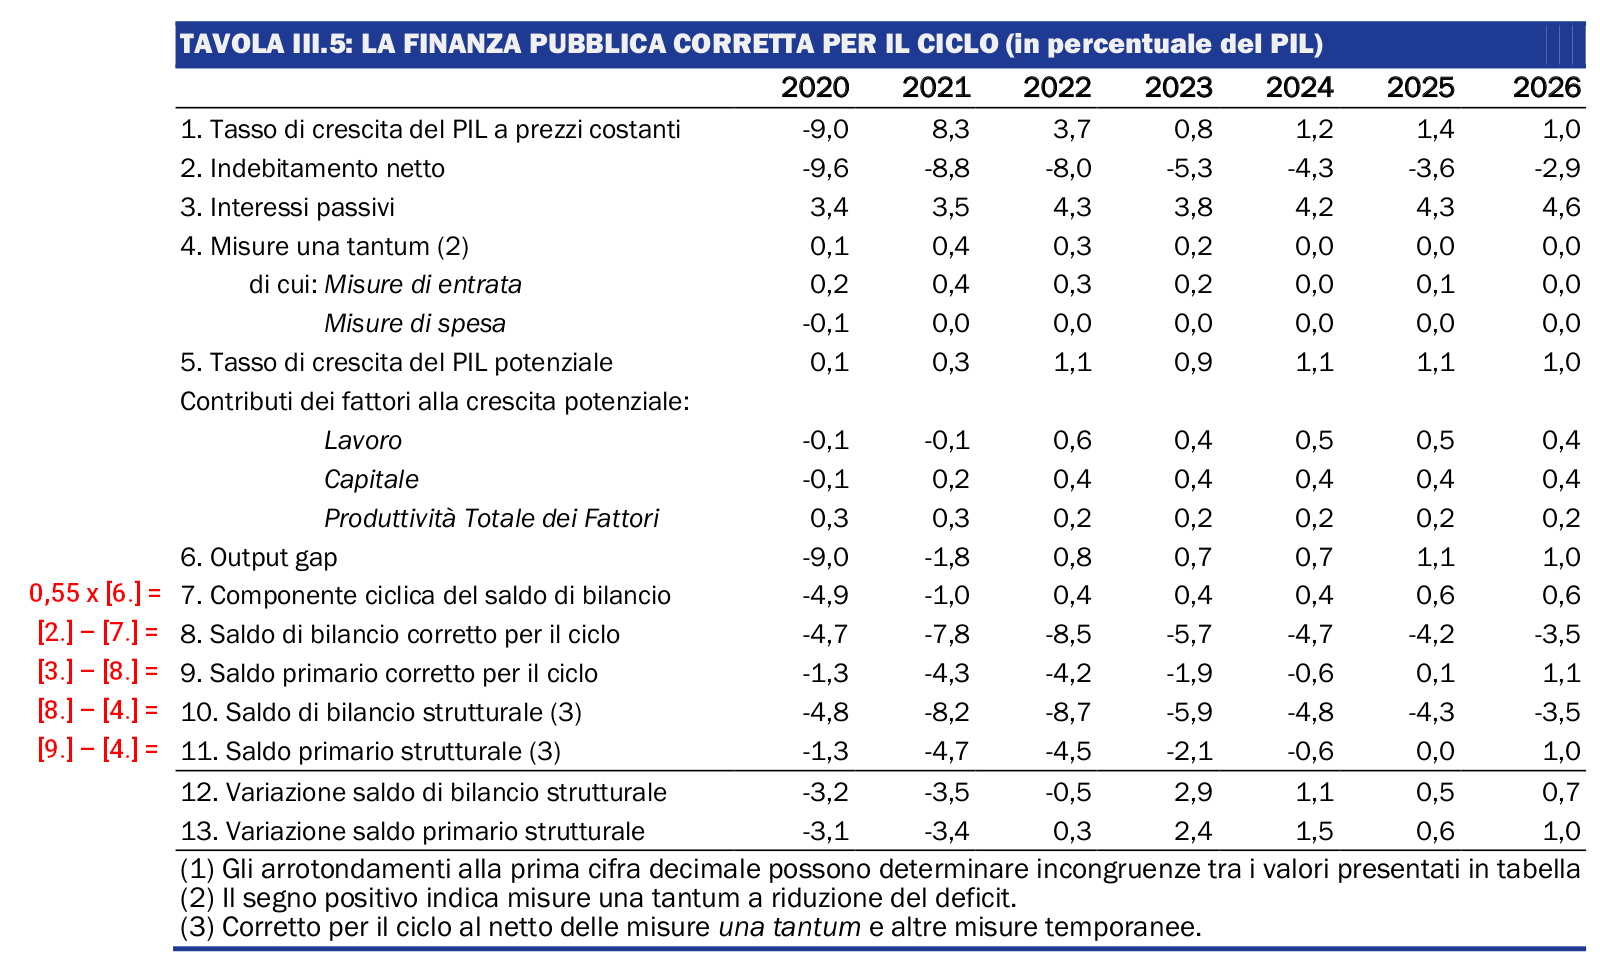
\includegraphics[width=\textwidth]{./figure/NADEF-2023-Tabella-III-5.png}
  \end{figure}

\vspace{-3mm}
\tiny Fonte: →\href{https://www.dt.mef.gov.it/export/sites/sitodt/modules/documenti\_it/analisi\_progammazione/documenti\_programmatici/nadef\_2023/NADEF-2023.pdf}{Nota di aggiornamento al DEF 2023}
\end{frame}

%%%%%%%%%%%%%%%%%%%%%%%%%%%%%%%%%%%%%%%%%%%%
\begin{frame}{Gli scostamenti rispetto alle regole UE}

  \vspace{-3.5mm}
  \begin{figure}[htbp]
    \centering
    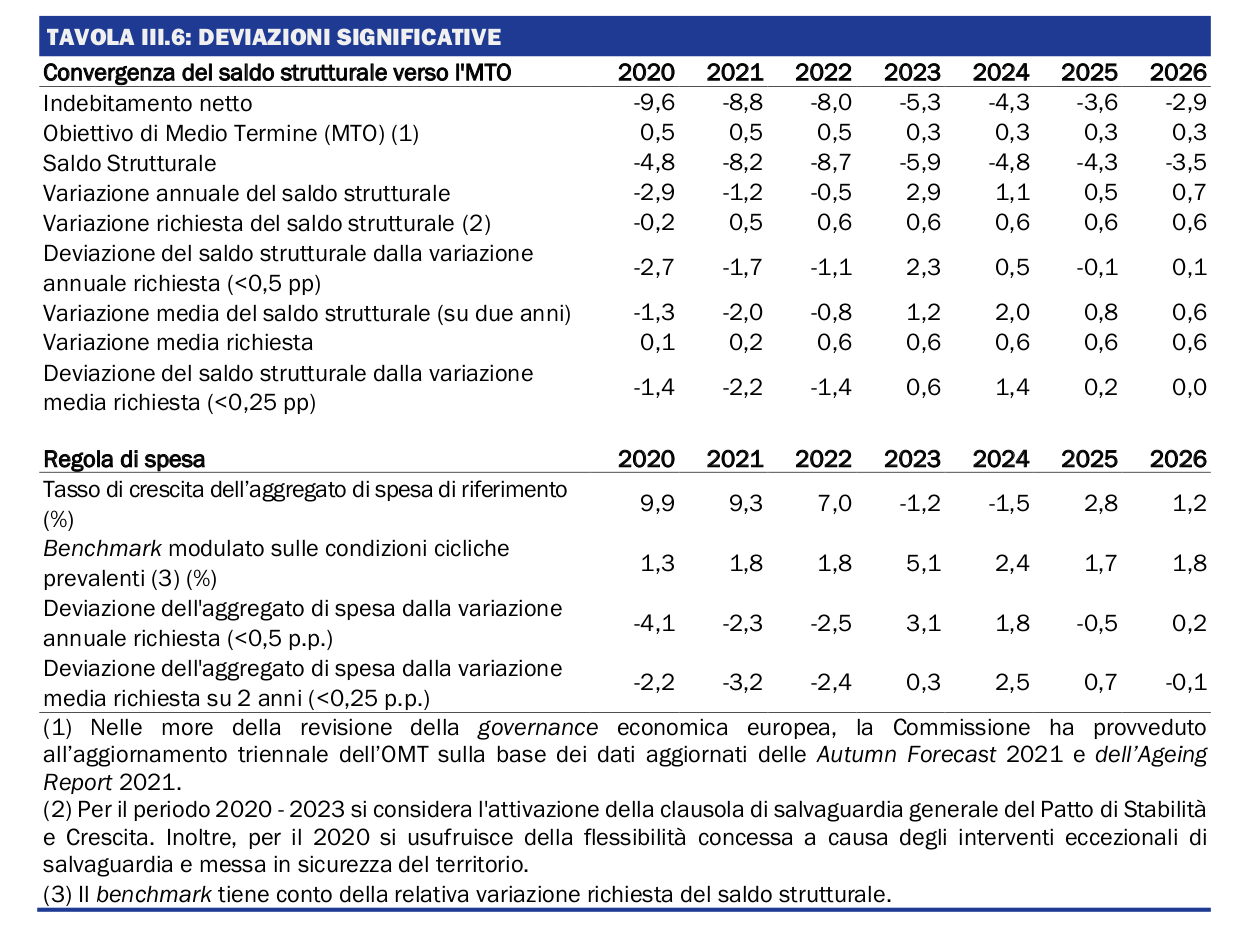
\includegraphics[height=7.5cm]{./figure/NADEF-2023-Tabella-III-6.png}
  \end{figure}

  \vspace{-3mm}
  \tiny Fonte:
 →\href{https://www.dt.mef.gov.it/export/sites/sitodt/modules/documenti\_it/analisi\_progammazione/documenti\_programmatici/nadef\_2023/NADEF-2023.pdf}{Nota
    di aggiornamento al DEF 2023}
\end{frame}


%%%%%%%%%%%%%%%%%%%%%%%%%%%%%%%%%%%%%%%%%%%%
\begin{frame}{La manovra per il 2024}

  \begin{columns}
    \begin{column}{.75\columnwidth}
      \vspace{-3mm}
      \begin{figure}
        \centering
        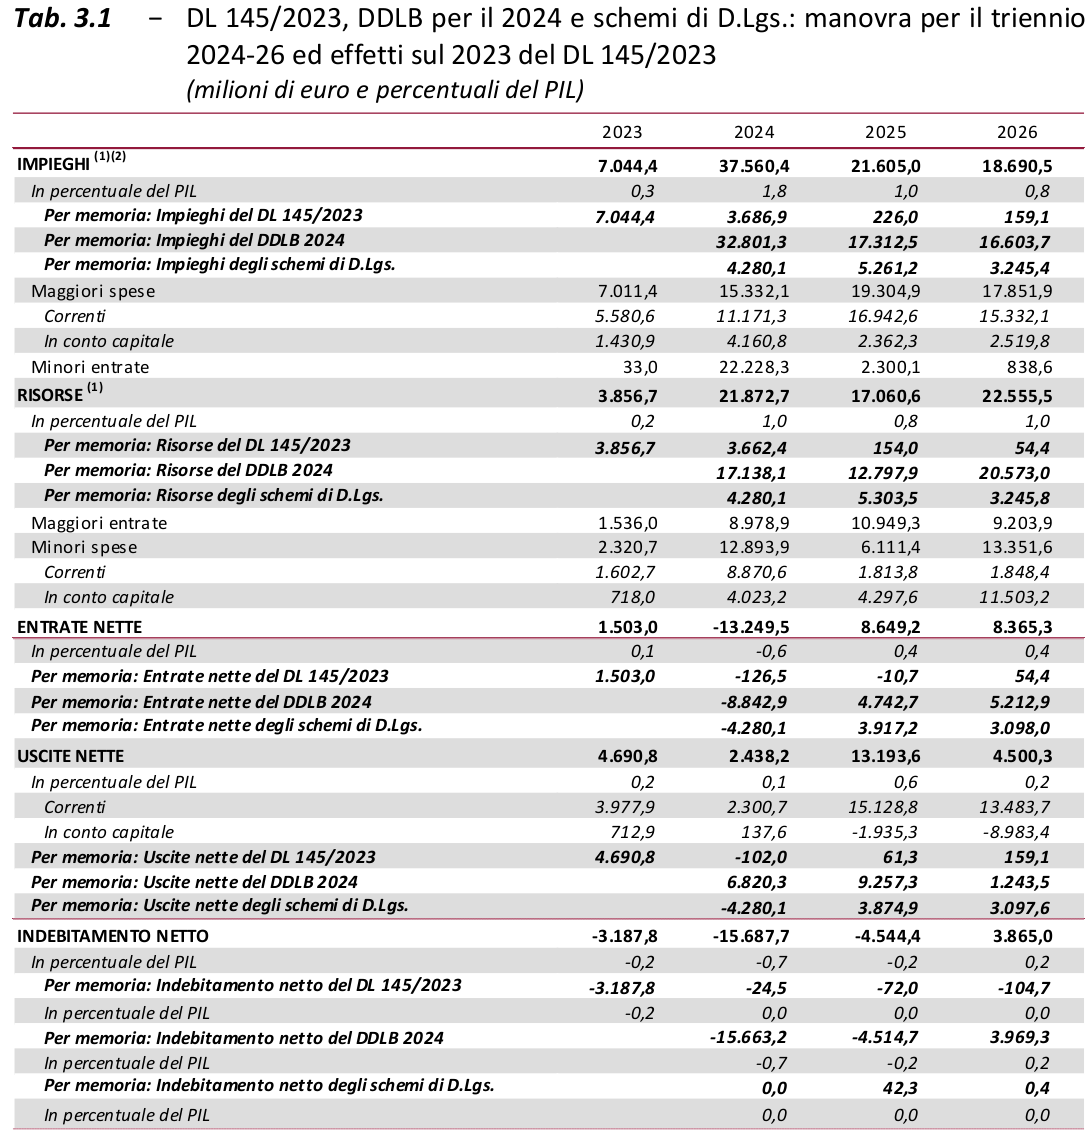
\includegraphics[height=7.5cm]{./figure/audizione-UPB-DDL-bilancio-2024-tab-3-1.png}
      \end{figure}
    \end{column}

    \begin{column}{.25\columnwidth}
      \footnotesize N.B. L'entità della manovra di bilancio è indicata come
      differenza rispetto alle previsioni tendenziali \alert{a legislazione
        vigente}
      
      \vspace{5mm}

      \tiny Fonte: →\href{https://www.upbilancio.it/wp-content/uploads/2021/11/Audizione-UPB-DDL-bilancio-2022.pdf}{Audizione del 23/11/2021 del Presidente dell'Ufficio Parlamentare di Bilancio} (Tab. 2.1)
    \end{column}
  \end{columns}
\end{frame}

\end{document}